\section{Mapning}
\label{mapning}
Et krav til denne opgave, er at lave et intelligent program, der kan køre rundt på en ukendt bane. Efter at bilen har kørt banen igennem, skal den kunne optimere sin kørsel. Dette betyder at den på de lange strækninger accelerer, men i svingene bremser ned til en sikker fart, der sikrer at den ikke falder af banen.

Til at udføre denne opgave skrives en algoritme, der køres første gang at bilen krydser den hvide linje. Denne algoritme opmåler banen ved at sammenholde den målte værdi af accelerometeret med faste værdier. Alt efter hvad accelerometerværdien er, beslutter algoritmen hvad der skal ske.
Figur \ref{testbanegraf2} viser den data bilen får fra accelerometeret. Dataen bliver sendt hver gang en vifte passerer forbi omdrejningssensoren.\\

\begin{figure}[h!]
\centering
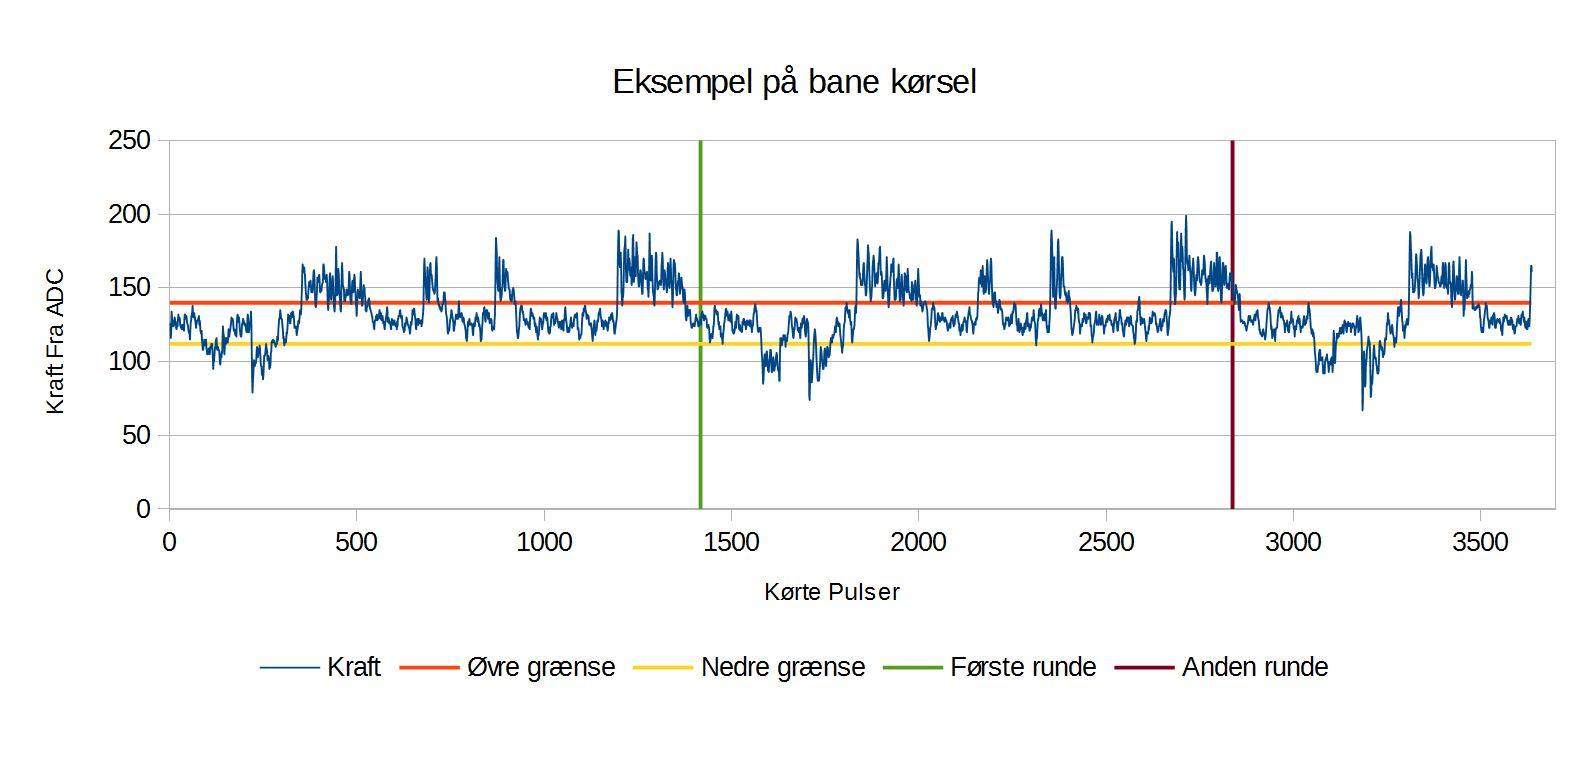
\includegraphics[scale=0.25]{./Graphics/banekorsel}
\caption{Graf over accelerometerdata fra testbanen. Billedet af testbane ses i bilag \ref{testbanebillede}}
\label{testbanegraf2}
\end{figure}

Når værdien fra accelerometeret er læst, behandles den af algoritmen, der bestemmer hvorvidt man er i et sving eller kører ligeud. Dette sker ved at sammenholde den læste værdi mod to faste værdier. Accelerometeret ligger, ved 0G, på ca $2,5 V$ (ADC værdien er 128 i decimal) men i praktisk lidt mindre. En ændring i g-kraften, som følge af et sving, vil øge eller sænke spændingen fra accelerometeret. Derfor tjekkes det om accelerometerværdien ligger uden for midterzonen. Midterzonen introduceres pga. støj ved lige ud kørsel. Dette område ligger mellem en ADC-værdi på 110 og 145, hvilket svarer til 2,148V – 2,832V. De to 
sikkerheds marginer ses på figur \ref{testbanegraf2} som den øvre grænse (Rød) og nedre grænse(Gul). Grænserne er fundet ud fra grafen.
Hvis man ser på et udsnit af et sving (Se figur \ref{180grader}), ses det at selv når den er i svinget, er der risiko for at den læste accelerometerværdi er under grænsen for hvornår et sving er detekteret. Dette diskuteres senere i afsnittet.\\

\begin{figure}[h!]
\center
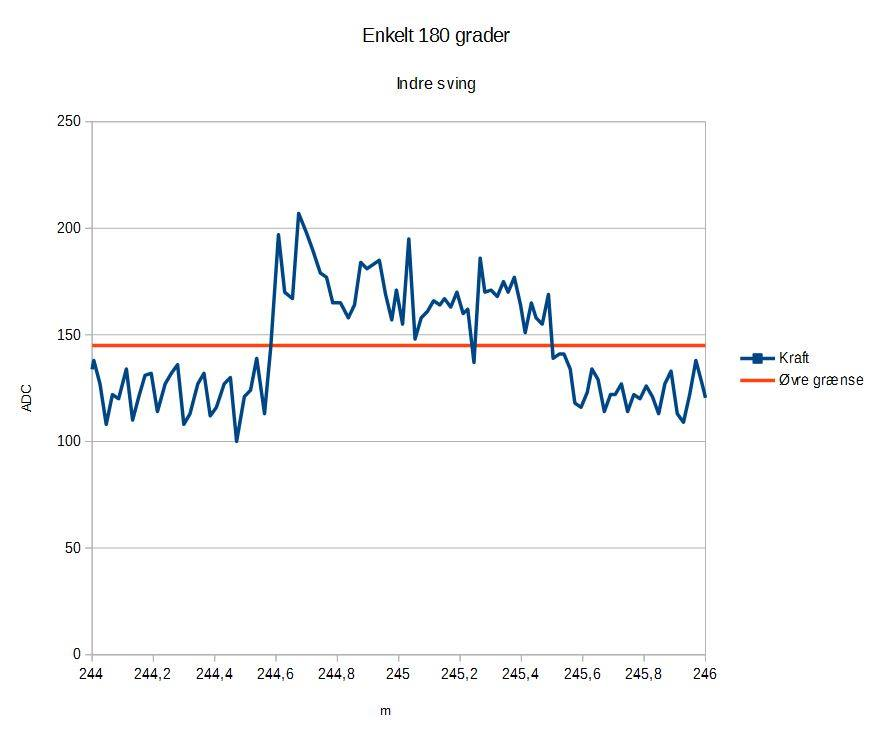
\includegraphics[scale=0.3]{./Graphics/Enkelt180grader}
\caption{Accelerometerværdi for et enkelt 180 grader sving}
\label{180grader}
\end{figure}

På figur \ref{Stjerne} er de sorte stjerner steder hvor den dykker under den øvre grænse og derved kunne give et falsk indtryk om at der er to sving. Ved at undersøge forskellig køredata, ses det at der er op mod fem fejl i målingerne. Dette kompenseres der for i programmet, ved at dette først accepterer at bilen er i et sving, hvis der kommer syv på hinanden følgende målinger over den øvre grænse. Dette vil resultere i at bilen nu ved at den er i et sving. På samme måde skal der også være syv på hinanden følgende målinger under øvre grænse før programmet accepterer at bilen er ude af svinget igen. Denne metode bruges også til at finde sving der ligger under den nedre grænse. \\ 

En anden metode man kunne implementere for ekstra sikkerhed, er ved at teste hvor langt der er mellem to målte sving. Hvis afstanden er under 35 cm vil man kunne udelukke at der er tale om to sving men der i mod kun et. Grunden til dette er at der i følge reglerne mindst skal være en lige skinne mellem sving. Denne metode er ikke implementeret grundet prioritering.\\

\begin{figure}[h!]
\center
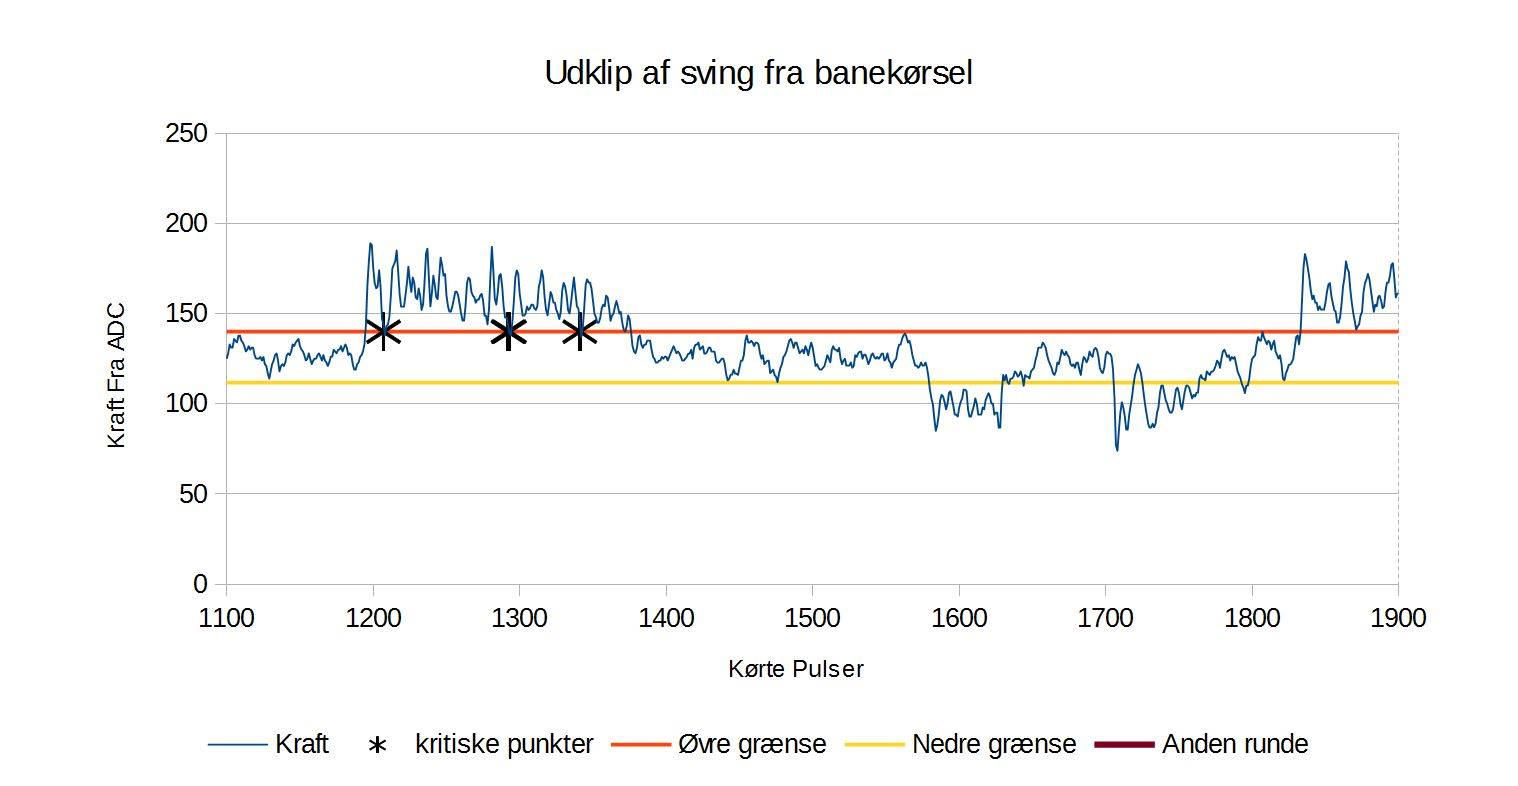
\includegraphics[scale=0.2]{./Graphics/sortestjerne}
\caption{Udklip af testbane data}
\label{Stjerne}
\end{figure}

